\section{System Description}

\subsection{Feasible space}
As in \cite{sun2014escaping}, a \textit{mission space}, $\Omega$, is defined as a simple polygon 
\cite{weissteinsimplepolygon}.
Within the mission space there exists $N_{o}\geq 0$ obstacles, each one of which is defined as a simple polygon.
The set of all obstacles, $\mathcal{O}$, is defined according to \eqref{obstacle_set_def}.
\begin{equation}\label[eq]{obstacle_set_def}
  \mathcal{O} = \begin{cases}
    \{o_{0}\hdots o_{N_{o}-1}\} &, N_{o} > 0\\
    \emptyset &, N_{o} = 0\\
  \end{cases}
\end{equation}
The obstacles in $\mathcal{O}$ constrains the movement of entities within the mission space, as it is not possible to
penetrate the boundary of an obstacle. Due to this, once an entity is inside $\Omega$, it is constrained to be positioned within
$\Omega$ and outside $\mathrm{int}(o)\;\forall\;o\in\mathcal{O}$. From this we define the \textit{feasible space}, $\mathcal{F}$, as
all points where it is possible to place an entity:
\begin{equation}\label[eq]{feasible_space_def}
  \mathcal{F} = \{\mathbf{y}\in\mathbb{R}^{2}: \mathbf{y}\in\Omega,\;\mathbf{y}\notin\mathrm{int}(o)\;\forall\;o\in\mathcal{O}\} = \Omega\setminus\bigcup_{o\in\mathcal{O}}\mathrm{int}(o)
\end{equation}

\subsection{Agent}
We define an \textit{agent} and its properties in a similar manner as in \cite{sun2014escaping}.
An agent, denoted by an index $a$, is defined by its position $\mathbf{x}_{a}\in\mathbb{R}^{2}$ and 
its maximum range of communication $r_{a}$. From this we define the communication disk of agent $a$:
\begin{equation}
  D_{a} = \{\mathbf{y}\in\mathbb{R}^{2}: \norm{\mathbf{x}_{a} - \mathbf{y}}\leq r_{a}\}
\end{equation}
Assuming line-of-sight (LoS) communication, meaning an agent cannot communicate with an entity if there is an obstacle or a mission space wall between them, we define the \textit{visible set} of agent 
$a$:
\begin{equation}\label[eq]{visible_set_def}
  V_{a} = \{\mathbf{y}\in\mathbb{R}^{2}:\mathbf{y}\in D_{a}, \lambda\mathbf{y} + (1-\lambda)\mathbf{x}_{a}\in\mathcal{F}\;\forall\;0\leq\lambda\leq 1\}
\end{equation}
The counterpart to the visible set, called the invisible set of agent $a$, is simply defined as:
\begin{equation}
  U_{a} = \mathcal{F}\setminus V_{a}
\end{equation}
An example of the visible set for an agent is show in \figref{vis_set_example}.

The probability of an agent $a$ being able to communicate with another entity positioned at a point $\mathbf{y}$, from now on called
the local probability of agent $a$, is defined according to:
\todo{Find notation for $\mathbb{R}^{5}$ with non-negative values in last dimension}
\begin{equation}\label[eq]{local_prob}
  \hat{p}:\mathbb{R}^{2}\rightarrow [0, 1]\quad\hat{p}(\mathbf{x}_{a}, \mathbf{y}) = \begin{cases}
    p(\norm{\mathbf{x}_{a}-\mathbf{y}}) &, \mathbf{y}\in V_{a}\\
    0 &, \mathbf{y}\in U_{a}
  \end{cases}
\end{equation}
Where $p(\cdot)$ is a non-increasing function of its argument.
\begin{figure}[H]
  \centering
  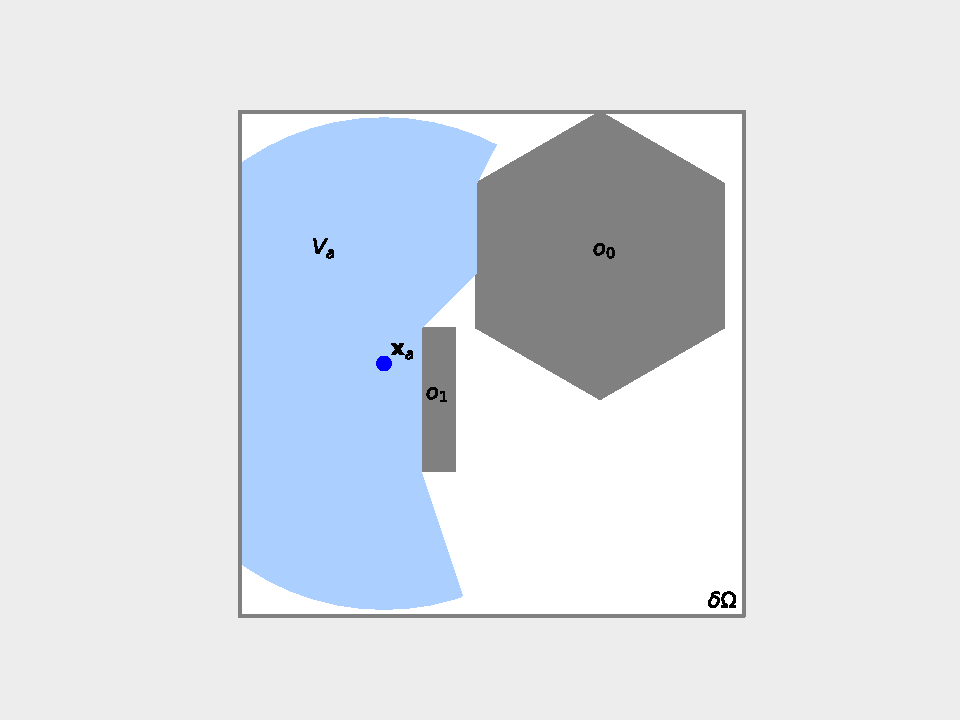
\includegraphics[width=\textwidth]{figs/vis_set_example.pdf}
  \caption{Visible set (light blue) for the agent placed at $\mathbf{x}_{a}$ in a rectangular mission space $\Omega$ with two obstacles ($\mathcal{O} = \{o_{0}, o_{1}\}$)}
  \label[fig]{vis_set_example}
\end{figure}
\todo{Update figure: $\mathbf{s}_{i}$ should be $\mathbf{x}_{a}$}
\subsection{Swarm}
A \textit{swarm}, $\mathcal{S}$ of size $N$ is a set of agents $\{a_{0}\hdots a_{N-1}\}$. The state of the swarm is described by the state of its participants 
, and is expressed as vector $\mathbf{X}_{\mathcal{S}}\in\mathbb{R}^{2N}$ as shown in \eqref{swarm_state_def}.
\begin{equation}\label[eq]{swarm_state_def}
  \mathbf{X}_{\mathcal{S}} = \begin{bmatrix}
    \mathbf{x}_{a_{0}}\\\vdots\\\mathbf{x}_{a_{N-1}}
  \end{bmatrix},\quad\mathbf{X}_{\mathcal{S}, i} = \mathbf{x}_{a_{i}}
\end{equation}
The maximum radii of communication of the swarm are represented as the vector $\mathbf{r}\in\mathbb{R}^{N}$ as shown in \eqref{swarm_radii_def}.
\begin{equation}\label[eq]{swarm_radii_def}
  \mathbf{r}_{\mathcal{S}} = \begin{bmatrix}
    r_{a_{0}}&\hdots&r_{a_{N-1}}
  \end{bmatrix}^{T}
\end{equation}
Assuming that the distributions for all agents in the swarm are independent lets us use (7) in \cite{10.2307/24304959} to express 
the probability of $n$ members in the swarm, $\mathcal{S}$, being able to communicate with an entity at a point $\mathbf{y}$:
\begin{equation}\label[eq]{Phi_def}
  \Phi^{n}(\mathbf{X}_{\mathcal{S}}, \mathbf{y}) = \sum_{A\in Comb(\mathcal{S}, n)}\prod_{a\in\mathcal{A}}\hat{p}(\mathbf{x}_{a}, \mathbf{y})\prod_{a\in\mathcal{S}\setminus\mathcal{A}}\big(1-\hat{p}(\mathbf{x}_{a}, \mathbf{y})\big)
\end{equation}
Later we will use the probability of \textit{at least} n members in a swarm beign able to communicate with an entity placed at $\mathbf{y}$, which is defined as:
\begin{equation}\label[eq]{more_than_n_prob}
  \Phi^{n^{+}}(\mathbf{X}_{\mathcal{S}}, \mathbf{y}) = 1 - \sum_{i=0}^{n-1}\Phi^{i}(\mathbf{X}_{\mathcal{S}}, \mathbf{y})
\end{equation}